\chapter{Diseño del sistema}

\section{Arquitectura general}

La arquitectura se diseña para evitar que el modelo de lenguaje responda directamente a una pregunta financiera sin cálculo verificable. El flujo separa tres responsabilidades generativas y varias capas deterministas de control.

El usuario formula una consulta en lenguaje natural. El sistema valida que existan tickers, fechas o periodo, intervalo y rutas a CSV locales. Después intervienen tres agentes LLM: el primero planifica el análisis, el segundo genera código Python y el tercero interpreta resultados ya calculados.

Entre la generación de código y la interpretación final se sitúa una capa de validación y ejecución controlada. Esta capa revisa el contrato del script, limita operaciones permitidas, ejecuta sobre datos históricos locales y captura la salida JSON. Así, las cifras no proceden de texto libre del modelo, sino de código ejecutado sobre datos trazables.

\begin{figure}[H]
\centering
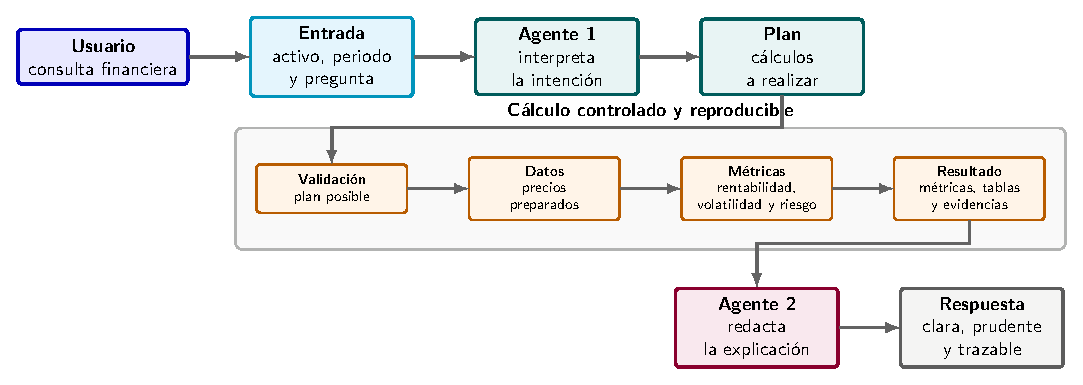
\includegraphics[width=0.96\textwidth]{figures/figura_5_1_usuario_final_v1.pdf}
\caption{Arquitectura general del sistema desde la consulta del usuario hasta la respuesta trazable.}
\label{fig:arquitectura_usuario_final}
\end{figure}

\begin{table}[H]
\centering
\small
\begin{tabularx}{\textwidth}{L{0.23\textwidth}L{0.30\textwidth}Y}
\toprule
\textbf{Bloque} & \textbf{Responsabilidad} & \textbf{Salida esperada} \\
\midrule
Entrada validada & Comprobar consulta, activos, fechas, intervalo y CSV. & Estructura de entrada procesable. \\
Agente 1 & Planificar: interpretar la consulta, elegir nivel A/B/C y definir métricas y salidas. & Plan analítico JSON, sin cifras inventadas. \\
Agente 2 & Generar código Python ajustado al contrato. & Script autocontenido que calcula sobre CSV locales. \\
Validación y ejecución & Revisar seguridad, ejecutar y capturar salida. & JSON con métricas, tablas, datos visuales si proceden y limitaciones. \\
Agente 3 & Explicar resultados ya calculados. & Respuesta final en español, prudente y sin recomendación de inversión. \\
\bottomrule
\end{tabularx}
\caption{Responsabilidades principales de la arquitectura.}
\label{tab:responsabilidades_arquitectura_general}
\end{table}

La trazabilidad es una propiedad transversal. El sistema conserva la pregunta, el plan, el código generado, la salida ejecutada, los errores y la respuesta final. Esta información permite repetir pruebas y localizar en qué fase aparece un problema.

\section{Nodos del flujo}

El flujo implementado puede entenderse como una cadena de nodos:

\begin{itemize}
    \item \textbf{Validación de entrada}: rechaza consultas vacías, fechas inválidas, ausencia de tickers o CSV inexistentes.
    \item \textbf{Agente 1: planificación}: identifica nivel A/B/C, objetivo analítico, métricas, columnas necesarias y salidas esperadas.
    \item \textbf{Agente 2: generación de código}: produce un script Python completo que lee un payload, calcula y emite JSON.
    \item \textbf{Validación de seguridad}: comprueba estructura, importaciones, lectura de entrada y salida JSON antes de ejecutar.
    \item \textbf{Reparación asistida}: si el script falla o se rechaza, puede pedirse una versión corregida que vuelve a validarse.
    \item \textbf{Ejecución controlada}: ejecuta el script en proceso separado sobre datos locales.
    \item \textbf{Compactación}: reduce salidas largas antes de enviarlas al agente interpretador, manteniendo la salida completa como evidencia.
    \item \textbf{Agente 3: interpretación}: redacta la respuesta final usando únicamente resultados ya calculados.
\end{itemize}

Esta separación permite diagnosticar fallos con precisión. Un caso puede detenerse por entrada inválida, configuración LLM, planificación incompleta, código no seguro, error de ejecución o fallo de interpretación.

\section{Contrato del código generado}

El contrato del código generado es la interfaz entre el modelo y la capa determinista. El script debe:

\begin{itemize}
    \item definir \texttt{main()};
    \item leer el payload mediante \texttt{Path(sys.argv[1]).read\_text};
    \item usar cargadores internos para los CSV;
    \item limitarse a importaciones permitidas;
    \item calcular métricas sobre datos históricos locales;
    \item devolver un único JSON por \texttt{stdout};
    \item incluir limitaciones cuando una métrica no pueda calcularse.
\end{itemize}

El script no redacta la respuesta final. Su responsabilidad es producir resultados estructurados: métricas, tablas, datos visuales en JSON si se solicitan y avisos de limitación. El agente de interpretación se encarga después de convertir esa salida en lenguaje natural.

\section{Gestión de errores}

Los errores se separan por origen: entrada, configuración del modelo, formato JSON, seguridad del código, ejecución e interpretación. El sistema no oculta estos fallos bajo una respuesta aparente. Si no puede completar una fase, devuelve un estado controlado y conserva el detalle del error.

Esta gestión es especialmente importante en un sistema con generación de código. Un fallo de cuota o red no significa mala planificación financiera; un código rechazado no equivale a una mala interpretación; y una ejecución correcta puede requerir todavía una respuesta final más clara. Separar los estados permite evaluar el sistema como ingeniería, no sólo como conversación.
